\documentclass[a4paper]{article}
\usepackage{geometry}
\usepackage[utf8]{inputenc}
\usepackage[T1]{fontenc}
\usepackage[bookmarks,colorlinks]{hyperref}
\usepackage[french]{babel}
\usepackage{pdflscape}
\usepackage{graphicx}

\title{Rapport du projet de Technologies Objets}
\author{Maxime Arthaud \and Korantin Auguste \and Martin Carton}
\date{11 juin 2013}

\begin{document}
\maketitle

\section{Introduction}
  Ce projet consiste en la création d'une interface utilisateur permettant de
  gérer une scène 3D et à la réalisation d'un moteur de rendu par lancé de
  rayons.

  Comme expliqué dans le rapport d'analyse, nous avons décidé de nous découper
  le travail, de façon à ce qu'une personne fasse l'interface graphique,
  une autre le parseur de fichier et l'écriture d'images au format PPM, et une
  autre travaille particulièrement sur le cœur du raytracer.

\section{Architecture}
  Le projet est donc constitué de deux programmes distincts:
  \begin{description}
      \item[L'interface graphique] Qui devra permettre de créer simplement des
        fichiers représentant des scènes, à passer à notre raytracer.
      \item[Le raytracer] Qui, à partir d'un fichier représentant une scène,
        devra générer un rendu, dans le format d'image de notre choix.
  \end{description}


  \subsection{Interface graphique}
    Maxime ?

    \begin{figure}[p]
      \centerline{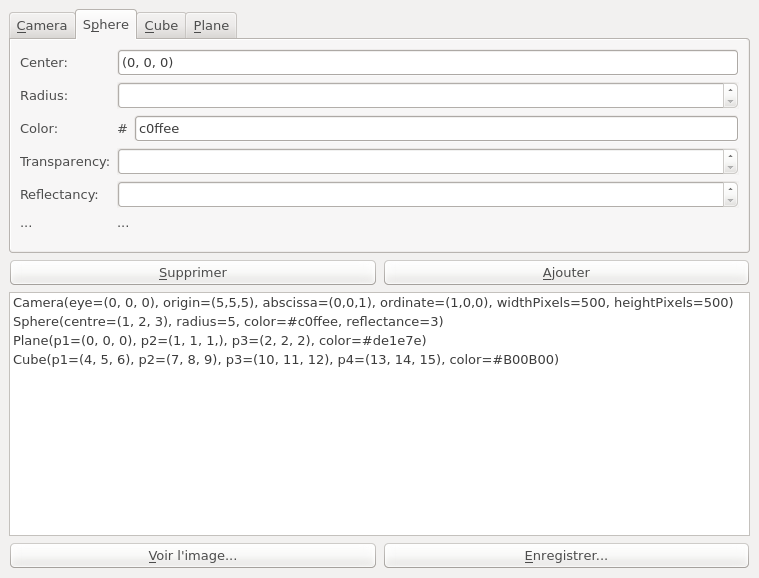
\includegraphics[width=1.2\textwidth]{gui.png}}
    \caption{Interface graphique\label{fig:gui}}
    \end{figure}

  \subsection{Raytracer}
    Pour créer le raytracer, nous avons convenu d'architecturer notre programme
    selon le diagramme de classes suivant présenté en figure \ref{fig:uml}.

    \newgeometry{width=1.3\linewidth}
    \begin{landscape}
      \thispagestyle{empty}
      \begin{figure}[p]
        \makebox[\paperwidth][c]{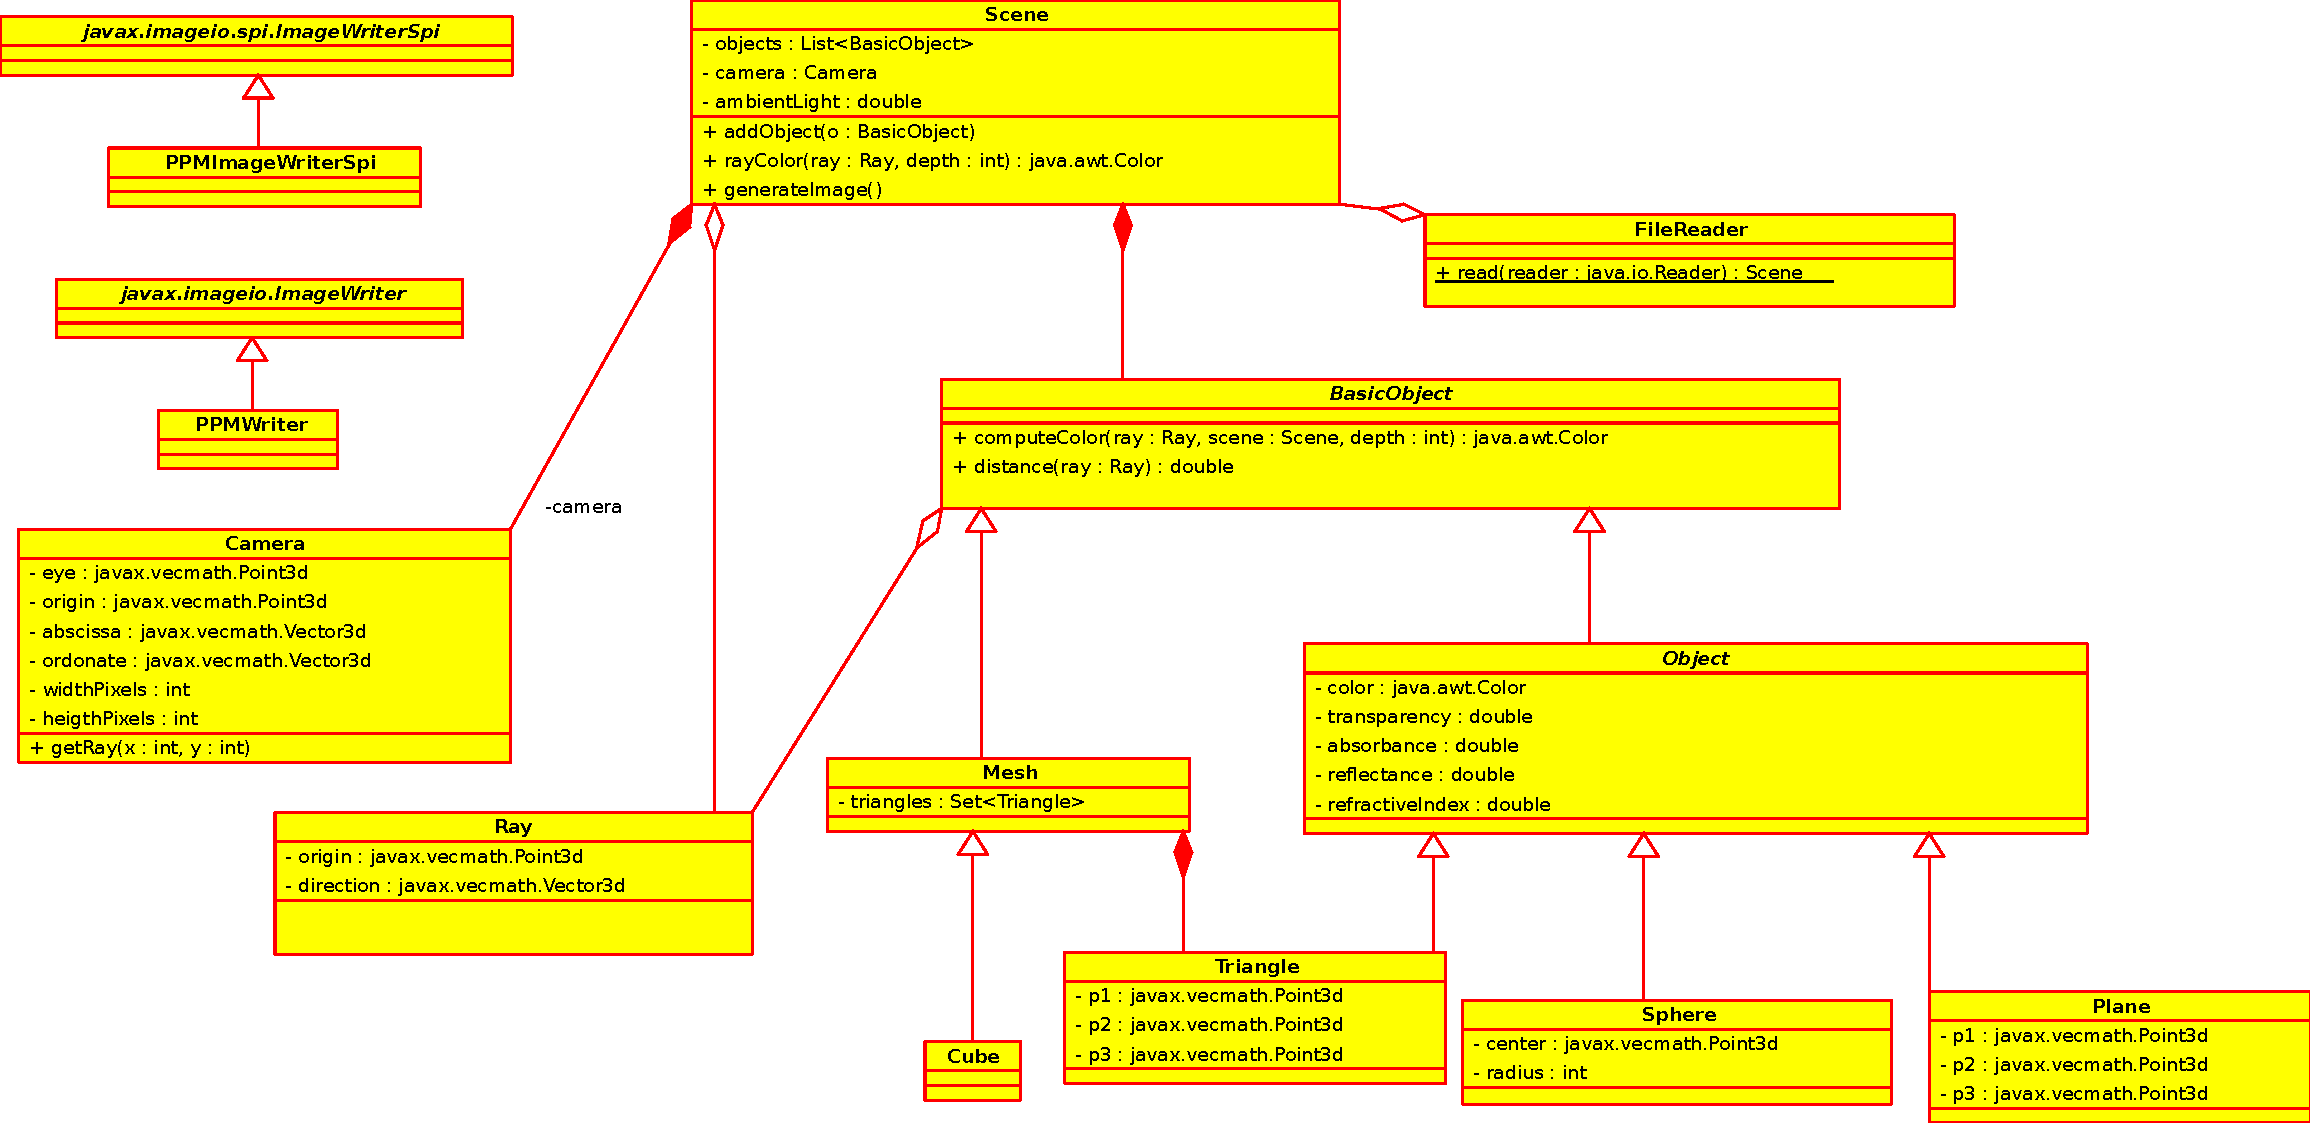
\includegraphics[width=25cm]{uml.pdf}}
        \caption{Diagramme UML\label{fig:uml}}
      \end{figure}
    \end{landscape}
    \restoregeometry

    Ainsi, l'objet scène dispose d'une méthode pour calculer la couleur d'un
    rayon passé en paramètre.
    Pour le faire, il va regarder quel objet va intersecter avec le rayon en
    premier, et appeler la méthode \verb+computeColor+ de l'objet en question.

    Cette méthode, définie dans la classe \verb+Object+, va faire tous les
    calculs nécessaires pour calculer les différentes composantes. Pour cela,
    elle peut même appeler à nouveau la méthode \verb+rayColor+ de la classe
    scène, sur les rayons réfléchis ou réfractés.
    Dans ces calculs, elle va appeler la méthode \verb+normal+, qui va donner
    la normale au point d'intersection du rayon avec l'objet, méthode qui sera
    définie dans des sous-classes, en fonction de l'objet.
\end{document}

